%% This is file `DEMO-TUDaReport.tex' version 3.35 (2023-12-11),
%% it is part of
%% TUDa-CI -- Corporate Design for TU Darmstadt
%% ----------------------------------------------------------------------------
%%
%%  Copyright (C) 2018--2023 by Marei Peischl <marei@peitex.de>
%%
%% ============================================================================
%% This work may be distributed and/or modified under the
%% conditions of the LaTeX Project Public License, either version 1.3c
%% of this license or (at your option) any later version.
%% The latest version of this license is in
%% http://www.latex-project.org/lppl.txt
%% and version 1.3c or later is part of all distributions of LaTeX
%% version 2008/05/04 or later.
%%
%% This work has the LPPL maintenance status `maintained'.
%%
%% The Current Maintainers of this work are
%%   Marei Peischl <tuda-ci@peitex.de>
%%   Markus Lazanowski <latex@ce.tu-darmstadt.de>
%%
%% The development respository can be found at
%% https://github.com/tudace/tuda_latex_templates
%% Please use the issue tracker for feedback!
%%
%% If you need a compiled version of this document, have a look at
%% http://mirror.ctan.org/macros/latex/contrib/tuda-ci/doc
%% or at the documentation directory of this package (if installed)
%% <path to your LaTeX distribution>/doc/latex/tuda-ci
%% ============================================================================
%%
% !TeX program = lualatex
%%

\documentclass[
	english,
	accentcolor=8b,
	type=intern,
	marginpar=false
	]{tudapub}

\hypersetup{
    colorlinks=true,
    linkcolor=orange,
    filecolor=magenta,      
    urlcolor=blue,
    % pdftitle={Overleaf Example},
    }

\usepackage[ngerman, main=english]{babel}
\usepackage[autostyle]{csquotes}
\usepackage{subcaption}
\usepackage{appendix}
\usepackage{datetime}
\usepackage{amsmath}
\usepackage{amssymb}
\usepackage{graphicx}
\usepackage{algorithm}
\usepackage{algpseudocode}
% Formatting for examples in this document. Generally, it's not necessary!
\let\file\texttt
\let\code\texttt
\let\pck\textsf
\let\cls\textsf
% \definecolor{tu8b}{HTML}{EC6500}

\begin{document}

\title{Refining Visual Question Answering with Selective Prediction on ViLT\\
}
\author{
Group E:\\
Muhammed Amjad Abdushakkoor\\
Ansh Prakash\\
Harshal Bhimani\\
}
\newdate{date}{08}{07}{2024}
\date{Deadline: \displaydate{date}}

\maketitle
%\tableofcontents

\section{Introduction}
According to \cite{agrawal2016vqavisualquestionanswering}, Visual Question Answering (VQA) models take an image and a question as inputs and produce a natural language answer. VQA integrates image understanding with text comprehension, involving tasks like object detection and reasoning \cite{agrawal2016vqavisualquestionanswering}. Several models have been developed, including Pythia, VisualBERT, and ViLT, which achieves this task.

For our work, we are focusing on Vision-and-Language Transformer (ViLT).
ViLT simplifies traditional Vision-and-Language Pre-training (VLP) by treating image processing similarly to text \cite{kim2021viltvisionandlanguagetransformerconvolution}. ViLT uses a transformer as a backbone, combining textual and visual data through layers to output a feature sequence \cite{kim2021viltvisionandlanguagetransformerconvolution}. It employs patch embedding for images and standard tokenization methods like WordPiece and BPE for text.

ViLT utilizes masked language modeling (MLM) and Image Text Matching (ITM) to enhance its capabilities in understanding and correlating images and text \cite{kim2021viltvisionandlanguagetransformerconvolution}. These mechanisms enable ViLT to generate answers from given image-question pairs with high accuracy.
However, it still faces an issue of being overconfident on OOD question-answer pairs. It simply doesn't know when it doesn't know.

\subsection{Selective prediction on VQA}
For VQA and other classification models, completely trusting their output may not be ideal as they don't provide any indicator about confidence on their predictions. They often try to find short-cut on training set. This situation is even worse when you consider how these models give a prediction out of their potential set of answers, even when its confidence in it is not good enough. There is generally no mechanism where it can say ‘I am not confident enough to answer’ or ‘I don’t know’ if its not trained well enough to give a confident output for a given input. \par
As illustrated in figure \ref{fig:selective_pred}, selective prediction works with the help of two main functions. Firstly, there is the function f(x) which is the main model that predicts the output text, when the image and question are given as inputs. Then, there is the selection function g(x), which determines whether the model must answer or abstain from answering \cite{whitehead2022reliablevisualquestionanswering}. \par
If g(x) let’s the model answer the given question, then the answer is shown to the user like its done normally. However, if the function makes the model abstain from answering, the prediction from the model is covered and an output such as ‘I don’t know’ or ‘Not confident enough to answer’ is shown to the user. \par
\begin{figure}[h]
\centering
\begin{subfigure}{.48\textwidth}
\centering
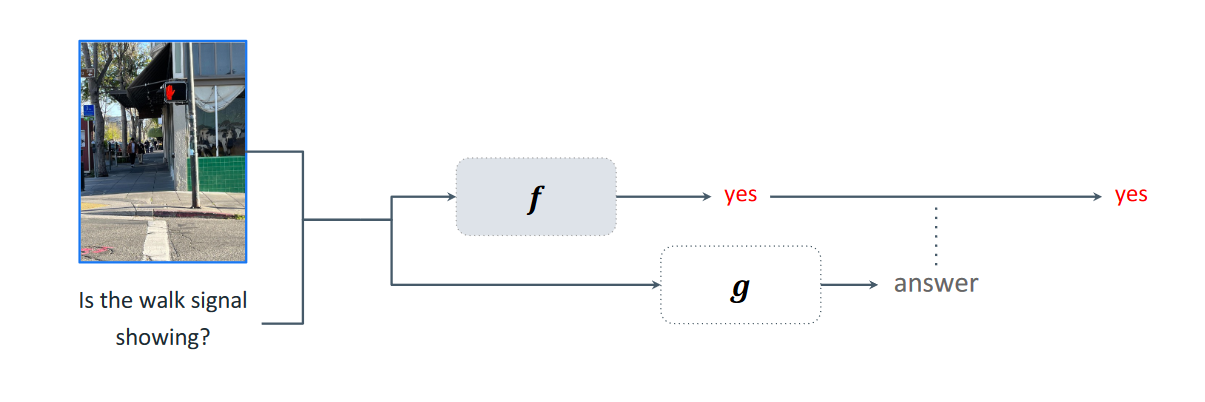
\includegraphics[width=0.8\textwidth]{figures/confidentv3.png}
\caption{When the selection function is confident}
\end{subfigure} \hfill
\begin{subfigure}{.48\textwidth}
\centering
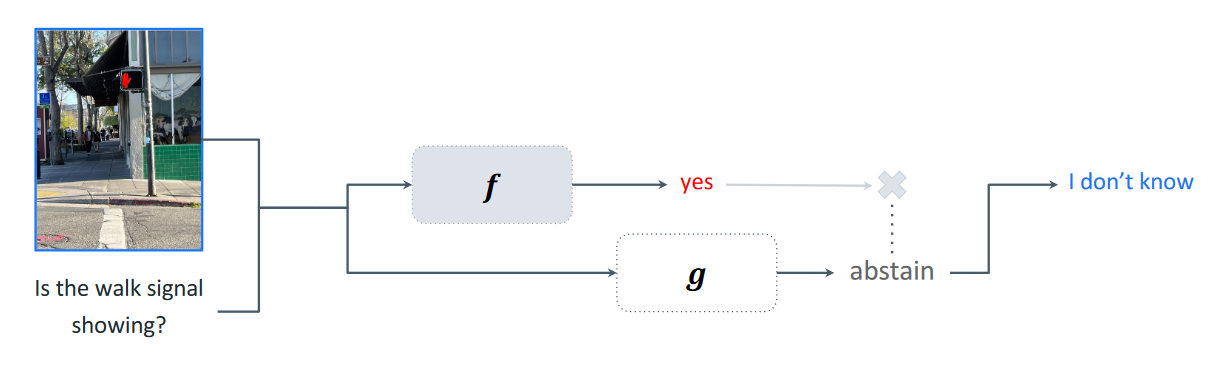
\includegraphics[width=0.8\textwidth]{figures/abstainv3.png}
\caption{When the selection function abstains}
\end{subfigure} \hfill
\caption{Working of selective prediction \cite{QuantificationLecture}} 
\label{fig:selective_pred}
\end{figure}


\subsection{Selection with Guaranteed Risk Control}
A selective classifier  is a pair (f, g), where f is a classifier, and g : X → {0, 1} is a selection
function, which serves as a binary qualifier for f as follows,


\[
(f, g)(x) \triangleq
\begin{cases} 
    f(x), & \text{if } g(x) = 1; \\
    \text{don't know}, & \text{if } g(x) = 0.
\end{cases}
\]

Thus, the selective classifier abstains from prediction at a point $x$ if and only if $g(x) = 0$. The performance of a selective classifier is quantified using coverage and risk. Fixing $P$, coverage, defined to be $\phi(f, g) = \mathbb{E}_P[g(x)]$
is the probability mass of the non-rejected region in $X$ \cite{whitehead2022reliablevisualquestionanswering}. The selective risk of $(f, g)$ is \[
R(f, g) = \mathbb{E}_P[\ell(f(x), y)g(x)] / \phi(f, g).
\]

We are given a classifier $f$, a training sample $S_m$, a confidence parameter $\delta > 0$, and a desired risk target $r^* > 0$. Our goal is to use $S_m$ to create a selection function $g$ such that the selective risk of $(f, g)$ satisfies
\[
\mathbb{P}_{S_m} \left\{ R(f, g) > r^* \right\} < \delta, \quad (2)
\]
where the probability is over training samples $S_m$ sampled i.i.d. from the unknown underlying distribution $P$. Among all classifiers satisfying , the best ones are those that maximize the coverage.


Yonatan et al. introduced this algorithm to find solution for the above eq \quad(2) using an additional confidence function.
In their work, they mentioned a confidence-rate function $\kappa_f : X \rightarrow \mathbb{R}_{+}$ for $f$.
The idea is that if $\kappa_f ( x_1) >= \kappa_f (x_2)$ then $f$ is more confident about $x_1$ then $x_2$
\hfill 

So, given a confidence parameter $\delta > 0$, and a desired risk target $r^* > 0$. Based on the training set, our goal is to learn a selection function $g$ such that the selective risk of the classifier $(f, g)$ satisfies (2).

For $\theta > 0$, the original authors' defined the selection function $g_\theta : X \to \{0, 1\}$ as
\[
g_\theta(x) = g_\theta(x \mid \kappa_f) \triangleq 
\begin{cases}
1, & \text{if } \kappa_f(x) \geq \theta; \\
0, & \text{otherwise}.
\end{cases} \quad (3)
\] 

\hfill

Additionally, \textit{empirical selective risk} with respect to the labeled sample $S_m$ is defined as follow:
\hfill
\[
\widehat{R}(f, g \mid S_m) \triangleq \dfrac {\frac{1}{m} \sum_{i=1}^{m} \ell(f(x_i), y_i) . g(x_i)}
{\quad \widehat{\phi}(f, g \mid S_m)}
\]

where $\widehat{\phi}$ is the empirical coverage, $\widehat{\phi}(f, g \mid S_m) = \frac{1}{m} \sum_{i=1}^{m} g(x_i)$.

Here, our objective is to minimize \textit{empirical selective risk} and at the same time try to have higher empirical coverage.
SGR Algorithm used in our work could be seen in \ref{alg:sgr}. 
Connecting back to  \quad(3), \ref{alg:sgr} will get us the $\theta$ value for the desired risk.

\begin{algorithm}
\caption{Selection with Guaranteed Risk (SGR)}
\label{alg:sgr}
\begin{algorithmic}[1]
\Procedure{SGR}{$f, \kappa_f, \delta, r^*, S_m$}
    \State Sort $S_m$ according to $\kappa_f(x_i)$ for $x_i \in S_m$ (and assume w.l.o.g. that indices reflect this ordering).
    \State $z_{\min} = 1$; $z_{\max} = m$
    \For{$i = 1$ to $k = \lceil \log_2 m \rceil$}
        \State $z = \left\lfloor \frac{z_{\min} + z_{\max}}{2} \right\rfloor$
        \State $\theta = \kappa_f(x_z)$ 
        \State $g_i = g_\theta$ 
        \State $\widehat{r}_i = \widehat{r}(f, g_i \mid S_m)$ \Comment{Estimate risk}
        \State $b^*_i = B^*(\widehat{r}_i, \delta/\lceil \log_2 m \rceil, g_i(S_m))$ \Comment{See Lemma 3.1 \cite{geifman2017selectiveclassificationdeepneural}}
        \If{$b^*_i < r^*$}
            \State $z_{\max} = z$
        \Else
            \State $z_{\min} = z$
        \EndIf
    \EndFor
    \State \textbf{Output} $(f, g_k)$ and the bound $b^*_k$.
\EndProcedure
\end{algorithmic}
\end{algorithm}

\subsubsection{Confidence function candidates}

There are different type of confidence functions that can be used for the purpose of SGR. Some of them are listed below. \par
\begin{itemize}
  \item \textbf{MaxProb}: This is the most basic kind of selection function and it uses the softmax probability of the prediction. Here, the idea is that the higher the value of the softmax, the more confident the model is about its predicted class. Therefore, this probability score can be compared with a certain threshold value to understand if the prediction made is strong enough to be shown \cite{whitehead2022reliablevisualquestionanswering}. If the probability score is greater than the threshold, it is shown to the user, or else the model is abstained from answering.
  \item \textbf{Platt Scaling}: The Platt scaling technique is only used for binary classifiers and is a technique to adjust the output of a classifier so it can give better probability estimates. Here, logits produced by the model are converted into probability scores and they are used in a simple logistic regression model to produce two variables a and b after its linear transformation. These variables are used to calibrate the logits and they are passed to a sigmoid function to produce the new probability scores \cite{guo2017calibrationmodernneuralnetworks}\cite{article}. 
  \item \textbf{Calibration with Matrix scaling}: Matrix scaling can be considered as a multi-class classifier version of Platt scaling as a matrix W is being used to calibrate the logits of the model. Therefore, instead of a linear regression based tranformation, the transformation yields: Wzi + b. Then softmax is applied to get the probabilities \cite{guo2017calibrationmodernneuralnetworks}.
  \item \textbf{Calibration with Vector scaling}: Vector scaling is a simpler version of matrix scaling where the matrix W is restricted to be diagonal. This means each class's logit is only scaled by a specific factor and shifted by a specific amount without mixing information between different classes\cite{guo2017calibrationmodernneuralnetworks}.
\end{itemize}
We are going to analyses on 'Maxprob' and 'Calibration with Vector scaling' with SGR \ref{alg:sgr}. Our expectation is that calibrated model should perform better as it reflects the model prediction confidence in sync with the reality.
 
\section{Related Work}
\label{sec:relwork}
\begin{itemize}
\item \textbf{Reliable Visual Question Answering: Abstain Rather Than Answer Incorrectly}: The paper \cite{whitehead2022reliablevisualquestionanswering} introduces abstention techniques to enhance VQA reliability by avoiding incorrect answers. The authors develop methods to improve both the accuracy and coverage of abstentions and propose the Effective Reliability metric for better VQA performance evaluation. This approach allows VQA models to maintain low error rates while increasing the number of questions they can confidently answer, setting a foundation for more reliable VQA systems.
\item \textbf{On Calibration of Modern Neural Networks}: In \cite{guo2017calibrationmodernneuralnetworks}, the concept of confidence calibration which is the accuracy of probability estimates in classification models are being investigated. The authors find that modern neural networks are poorly calibrated compared to older models and identify factors such as depth, width, weight decay, and Batch Normalization as influential. Through extensive experiments, they evaluate various post-processing calibration methods and determine that temperature scaling is highly effective for most datasets, providing practical guidance for improving calibration in neural networks.
\item \textbf{Improving Selective Visual Question Answering by Learning from Your Peers}: The paper \cite{dancette2023improvingselectivevisualquestion} enhances the ability of VQA models to abstain from answering when uncertain, especially with out-of-distribution (OOD) inputs. The proposed Learning from Your Peers approach trains selection functions using model predictions from distinct data subsets. This method significantly improves performance, achieving 32.92% 
\end{itemize}
\section{Main Contribution}
\label{sec:approach}
We will analyze selective prediction strategies on a ViLT model. Specifically the vilt-b32-finetuned-vqa model from dandelin will be used. This is a fine tuned model that was trained on the VQAv2 dataset and was introduced in \cite{kim2021viltvisionandlanguagetransformerconvolution}. \par
Moreover, we will specifically going into the testing of selective prediction using MaxProb, and calibration by vector scaling selection functions. The results from experimenting with the various techniques of selective prediction will be available in section \ref{sec:analysis}. \par
Our main contributions include:
\begin{itemize}
  \item Applying Selection with Guaranteed Risk (SGR) Algorithm \cite{geifman2017selectiveclassificationdeepneural} in multi-modal setting
  \item Experimenting with Calibrated logits in addition to MaxProb
\end{itemize}

\section{Experimental Setup}
\label{sec:experiments}

\textbf{Dataset}: We use the \href{https://visualqa.org/download.html}{VQAv2} dataset, which contains around 3,000 classes. Visual Question Answering (VQA) v2.0 is a dataset with open-ended questions about images that require an understanding of vision, language, and commonsense knowledge to answer.

We randomly divide the validation set into two equal halves: one for training and the other for testing risk and coverage.

\textbf{Correct Label Choice}: Since VQAv2 has 10 labels from different humans, we consider the label occurring the maximum number of times as the correct label. Our results and risk measures are based on this method of determining the correct label.

\textbf{Model}: We use the \href{https://huggingface.co/dandelin/vilt-b32-finetuned-vqa}{ViLT model fine-tuned on VQAv2}.

\textbf{Objective}: We aim to enable the model to abstain when it is not confident about its prediction while maximizing coverage. We employ the Selection with Guaranteed Risk (SGR) algorithm introduced by Yonatan et al. \cite{geifman2017selectiveclassificationdeepneural} and investigate whether \textit{calibrated logits perform better than vanilla logits}.

Yonatan et al. used the SGR algorithm in a unimodal setting with Maxprob as the confidence function. We extend this concept to a multimodal setup and experiment with calibrated logits using a vector-scaling method. Temperature scaling was not used as it does not change the order of softmax probabilities and is thus equivalent to the Maxprob method.

\textit{To find $\theta$ for the correct risk bound, we will apply the SGR algorithm \ref{alg:sgr}.}

\textbf{Flow}:
\begin{enumerate}
    \item Generate logits from the ViLT model using the validation dataset.
    \item Train a vector-scaling calibration model using these logits.
    \item Treat both the vanilla logits and the calibrated logits (after applying softmax and taking the maximum value) as confidence values.
    \item Create a list of confidence values and a boolean list where incorrect predictions are marked as 1.
    \item Feed these lists into the SGR algorithm \ref{alg:sgr}.
    \item Use the generated $\theta$ in equation (3) to create a rejection function.
    \item Determine $\theta$ for various risk values.
\end{enumerate}

\section{Results and Analysis}
\label{sec:analysis}
% Present the results (e.g., show tables and plots/figures) and elaborate on the key findings from your experiments. Discuss the performance of your approach(es), how it compares to the baselines, any notable results or trends observed, and how they align with your expectations. Include qualitative results to illustrate the successes and failures of your approach / compared approaches. 
% (An example of a table can be found in Table \ref{tab:modality_subset_results}. I personally can recommend \href{https://tablesgenerator.com/}{LaTeX table generator} to generate large tables.)
Observing the results in Table \ref{tab:max_prob_selective_prediction}, we see that the risk bound, \( b^* \), is always very close to the target risk, \( r^* \), for the Maxprob method. However, this is not the case with the vector-scaling method, which fails to find a reasonable risk bound at 2\% in Table \ref{tab:vec_scal_selective_prediction}.

Additionally, at 100\% desired risk, we reach the empirical risk without selective prediction.

We notice that coverage increases significantly as the desired risk increases. Surprisingly, vector-scaling calibration performs worse than vanilla logits according to our results. Nonetheless, our coverage values seem to be better than some of the current state-of-the-art work, such as that by \href{https://openaccess.thecvf.com/content/CVPR2023/papers/Dancette_Improving_Selective_Visual_Question_Answering_by_Learning_From_Your_Peers_CVPR_2023_paper.pdf}{Whitehead et al.}

Overall, we find that calibrated logits do not perform as well as vanilla logits, proving our hypothesis incorrect.


\begin{table}[h]
\begin{tabular}{|c|c|c|c|c|c|}
\hline
desired risk & train risk & train coverage & test\_risk & testcov& bounded risk \\ \hline
0.02 & 0.0173 & 0.3624 & 0.0177 & 0.3649 & 0.0200  \\
0.10 & 0.0957 & 0.6810 & 0.0980 & 0.6810 & 0.1000  \\
0.15 & 0.1453 & 0.8013 & 0.1420 & 0.8002 & 0.1500  \\
0.20 & 0.1950 & 0.9133 & 0.1940 & 0.9125 & 0.2000  \\
0.25 & 0.2448 & 0.9996 & 0.2432 & 0.9996 & 0.2500  \\
0.30 & 0.2444 & 1.0000 & 0.2442 & 1.0000 & 0.2496  \\
1.00 & 0.2440 & 1.0000 & 0.2446 & 1.0000 & 0.2491  \\
\hline
\end{tabular}
\caption{Risk control results with Maxprob for VQAv2 for $\delta = 0.001$ }
\label{tab:max_prob_selective_prediction}
\end{table}
\begin{table}[h]
\begin{tabular}{|c|c|c|c|c|c|}
\hline
desired risk & train risk & train coverage & test\_risk & testcov& bounded risk \\ \hline
0.02 & 0.0000 & 0.0000 & 0.0303 & 0.4585 & 0.9999  \\
0.10 & 0.0957 & 0.6785 & 0.0961 & 0.6796 & 0.1000  \\
0.15 & 0.1452 & 0.7909 & 0.1436 & 0.7905 & 0.1500  \\
0.20 & 0.1950 & 0.8976 & 0.1937 & 0.8975 & 0.2000  \\
0.25 & 0.2448 & 0.9996 & 0.2445 & 0.9997 & 0.2500  \\
0.30 & 0.2446 & 1.0000 & 0.2453 & 1.0000 & 0.2497  \\
1.00 & 0.2461 & 1.0000 & 0.2437 & 1.0000 & 0.2513  \\
\hline
\end{tabular}
\caption{Risk control results with vector-scaling calibration for VQAv2 for $\delta = 0.001$ }
\label{tab:vec_scal_selective_prediction}
\end{table}

\newpage
\section{Conclusions and Limitations}
\label{sec:conclusion}
We found that vector-scaling with SGR didn't provide any significant improvement over Maxprob as confidence-rate function. 
In extreme case, SGR algorithm failed to find a reasonable bounded risk for calibrated logits.
Moreover, the biggest limitation of our method is that we are trying to get confidence value from model itself.
In research, it has been shown that even after applying calibration, models are still overconfident on OOD data.
In future work, we should disentangle the method of getting confidence value from within the classifier itself.


\subsubsection{Our Learnings}
We have learned :
\begin{enumerate}
    \item Calibrating models with vector-scaling, temperature-scaling, and matrix-scaling
    \item Found a way find a $r^*$, such that it tries to balance risk and coverage
    \item Dissecting research paper and finding what could be relevant to solve a problem
    \item Coding practices required in a team
\end{enumerate}


% Summarize the main outcomes of your project. \textbf{Answer your research question}. Discuss what you have learned, the implications of your findings, and any potential future directions. Discuss any limitations of your work. Keep it concise and focus on the core takeaways, no need to be repetitive w.r.t. previous sections.

%\newpage
\bibliographystyle{abbrv}
\bibliography{references}

\appendix 

\section{GitHub Project Info {\color{red}(mandatory)}}
\textbf{GitHub Link}: \href{https://github.com/Amjad-MA5/Selective_Prediction_VQA}{GitHub} \par

\begin{itemize}
\item \textbf{Muhammed Amjad Abdushakkoor} - Amjad-MA5
\item \textbf{Ansh Prakash} - AnshPrakash
\item \textbf{Harshal Bhimani} - harshal912
\end{itemize}

\section{Individual Contributions {\color{red}(mandatory)}}


Muhammed Amjad has worked on the testing of various VQA models which led to the choosing of the model used in this paper. Also, he has developed the initial maxprob based selective prediction part of the topic. Moreover, he was tasked with writing most parts of the report. \par
Harshal Bhimani has worked on the development and testing of the maxprob and risk bound methodologies, ensuring the code structure for predictions, risk bound, and batch processing was robust. After confirming the model's workflow and outputs, he integrated batch processing and the risk bound components. \par

Ansh Prakash developed the hypothesis and implemented various critical modules. He generated the final experimental results presented in our report. Furthermore, he worked on various parts of the report. Additionally, he managed the team.

\section{Additional Content (optional)}
Here, you can include additional details, qualitative examples, etc., which you do not wish to include in the main report.

\end{document}
